\hypertarget{oauth_intro_oauth}{}\section{\-Introduction}\label{oauth_intro_oauth}
\-O\-Auth 2.\-0 is an open authorization protocol which enables applications to access each others data. \-For example, a game application can access a users data in the \-Facebook application etc. \-The following sections should give a basic overview of the \-O\-Auth 2.\-0 protocol.\hypertarget{oauth_roles}{}\section{\-Roles}\label{oauth_roles}
\-O\-Auth 2.\-0 defines four basic roles\-:
\begin{DoxyItemize}
\item \-The resource owner (or user)\-: \par
 \-The person (or application) that owns the data that is to be shared \par
\par

\item \-The resource server\-: \par
 \-The server responsible for storing and managing the resources \par
\par

\item \-The client applictation (or just client)\-: \par
 \-The application that requests access to the rescources stored on the resource server \par
\par

\item \-The authorization server\-: \par
 \-The server responsible for authorizing the client to access the protected resources, can be the same as the resource server
\end{DoxyItemize}\-Their interaction is illustrated in the following diagram\-:  
\begin{DoxyImage}
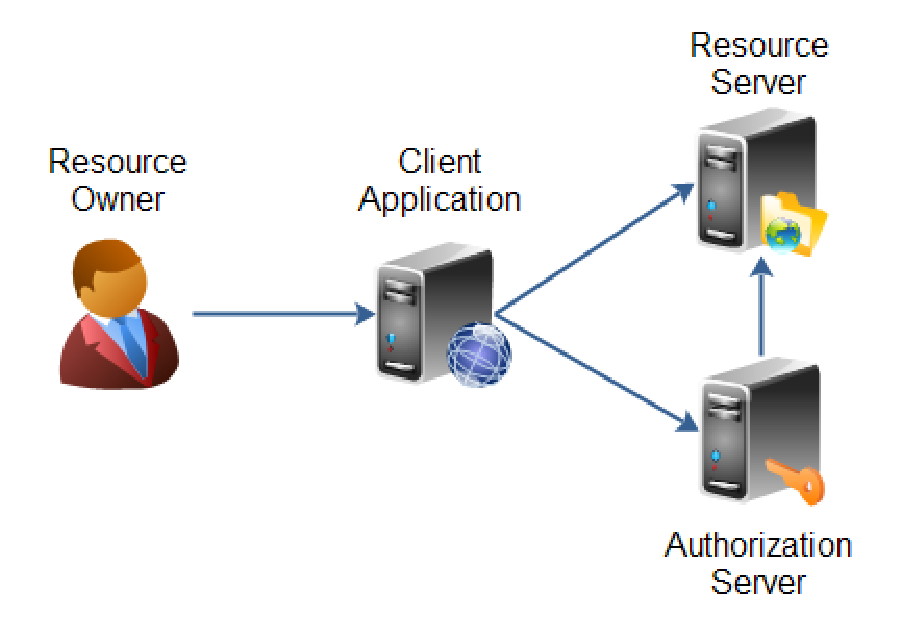
\includegraphics[width=10cm]{overview-roles}
\caption{\-Basic roles defined by \-O\-Auth 2.0}
\end{DoxyImage}
\hypertarget{oauth_flow}{}\section{\-Abstract Protocol Flow}\label{oauth_flow}
\-The basic flow of \-O\-Auth 2.\-0 (as shown in the diagram below) is as follows\-:

\-To get access to protected resources a client sends an authorization request to the resource owner(user). \-If the user grants authorization, the client gets an authorization grant, this grant can take different forms (see \hyperlink{oauth_grant}{\-Authorization \-Grant}) \par
 \-The client exchanges the grant for an access token at the authorization server. \par
 \-The access token can then be used by the client to access the protected resources.

 
\begin{DoxyImage}
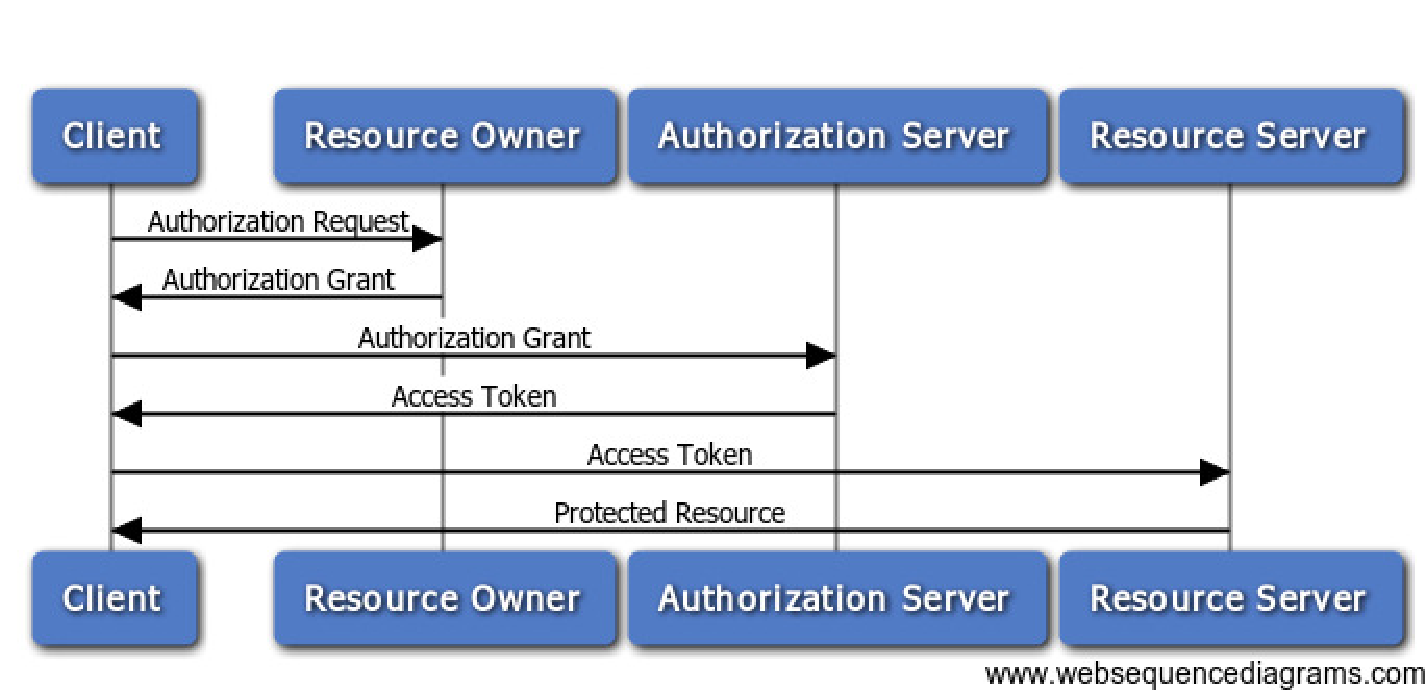
\includegraphics[width=10cm]{flow}
\caption{\-Abstract protocol flow}
\end{DoxyImage}
\hypertarget{oauth_auth}{}\section{\-Authorization}\label{oauth_auth}
\hypertarget{oauth_registration}{}\subsection{\-Registration}\label{oauth_registration}
\-Before the client can request access to protected resources, the client needs to register with the authorization server.\par
 \-During that process the client is assigned a unique client \-I\-D and a client secret.\par
 \-The client also registers a redirect \-U\-R\-I, which is where the user is redirected to, after granting/denying authorization.\par
\hypertarget{oauth_grant}{}\subsection{\-Authorization Grant}\label{oauth_grant}
\-O\-Auth 2.\-0 specifies the following four types of authorization grants\-:\hypertarget{oauth_authcode}{}\subsubsection{\-Authorization Code}\label{oauth_authcode}
\-Since this is the grant implemented in this application a more detailed explanation is required. \par
 \-The basic idea of this grant is as follows\-:
\begin{DoxyItemize}
\item \-The user accesses the client application (1)
\item \-The client app asks the user to log in via an authorization server (2)
\item \-The user is redirected to the authorization server by the client, the client also sends its client \-I\-D along (3)
\item \-After successful login via authorization server the user is asked if he/she wants to grant authorize the client to access the user data.\par
 \-The user is redirected to the registered redirect \-U\-R\-I of the client along with an authorization code (4, 5)
\item \-At the redirect \-U\-R\-I the client connects directly to the authorization server and sends its client \-I\-D, client secret and the authorization code.\par
 \-If all of the data is valid, the authorization server sends back an access token (6, 7)
\item \-This token is sent with every recource request and serves as authentication of the client and authorization to access the recources (10-\/13)
\end{DoxyItemize}

 
\begin{DoxyImage}
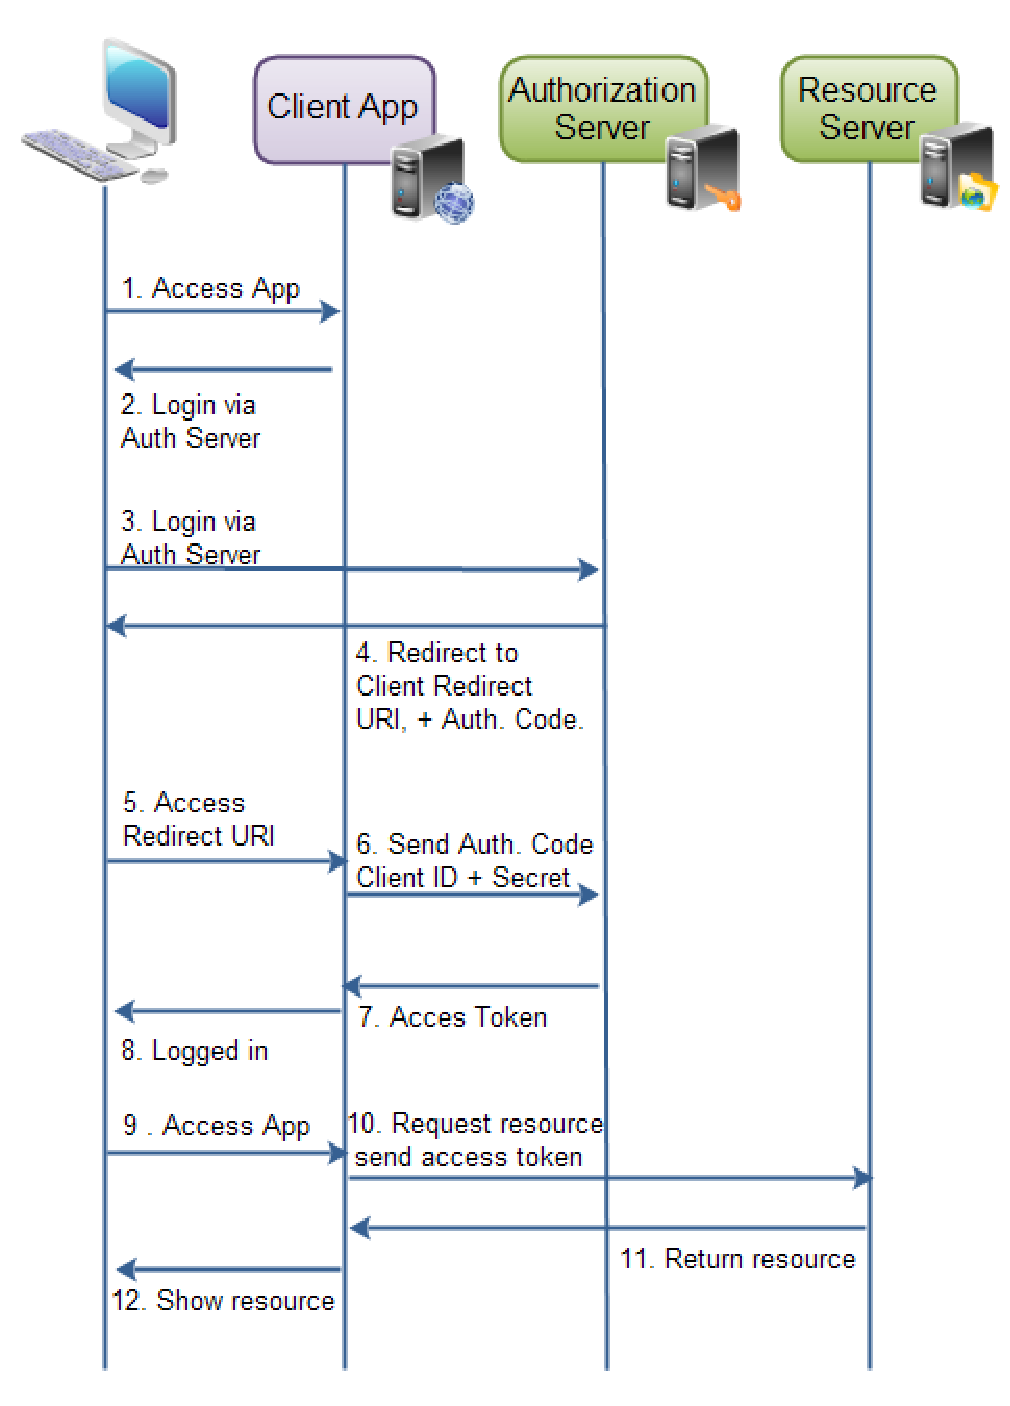
\includegraphics[width=8cm]{authorization-auth-code}
\caption{authorization code grant flow}
\end{DoxyImage}
\hypertarget{oauth_implicit}{}\subsubsection{\-Implicit}\label{oauth_implicit}
\-The implicit grant is similar to authorization code grant, the difference being that the authorization server sends an access token \par
 to the client immediatly after the client logged in and authorized the client.\hypertarget{oauth_ropc}{}\subsubsection{\-Resource Owner Password Credentials}\label{oauth_ropc}
\-This grant requires the user to give the own credentials to the client application, so that the client can use them to access the resources.\hypertarget{oauth_cc}{}\subsubsection{\-Client Credentials}\label{oauth_cc}
\-The authorization server exchanges an access token for client \-I\-D and client secret directly\hypertarget{oauth_endpoint}{}\subsection{\-Endpoint}\label{oauth_endpoint}
\-An endpoint is usually a \-U\-R\-I on a server, in the case of \-O\-Auth 2.\-0 these are\-:
\begin{DoxyItemize}
\item \-The authorization endpoint\-: \par
 \-The endpoint where the user logs in and grants/denies authorization to the client \par
\par

\item \-The redirect endpoint\-: \par
 \-The endpoint where the user is redirected to after granting/denying authorization \par
\par

\item \-The token endpoint\-: \par
 \-The endpoint where the client exchanges client \-I\-D, client secret and authorization code for an access token \par
\par

\end{DoxyItemize}

 
\begin{DoxyImage}
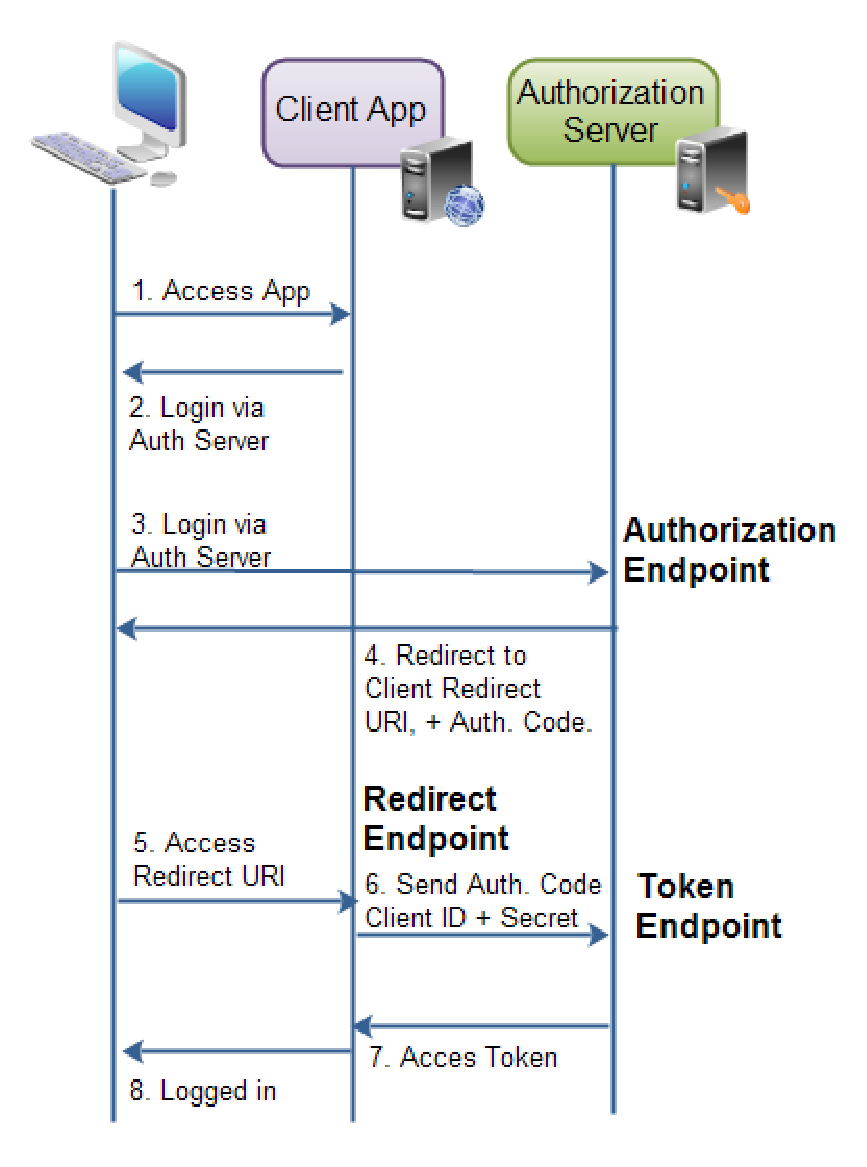
\includegraphics[width=7cm]{endpoints}
\caption{\-Endpoints defined by \-O\-Auth 2.0}
\end{DoxyImage}
 